
% Este documento LaTeX fue diseñado por profesores  del Departamento de Matemáticas 
% de la Universidad de Antioqua (http://ciencias.udea.edu.co/). Usted puede modificarlo
% y personalizarlo a su gusto bajo los términos de la licencia de documentación libre GNU.
% http://es.wikipedia.org/w/index.php?title=Licencia_de_documentaci%C3%B3n_libre_de_GNU&oldid=15717448

\documentclass[serif,9pt, t]{beamer}
\setbeamertemplate{navigation symbols}{}
\addtobeamertemplate{navigation symbols}{}{
    \insertframenumber/\inserttotalframenumber
}
\setbeamercolor{navigation symbols}{fg=black}
\usetheme{Warsaw}

\usepackage[utf8]{inputenc}
\usepackage[spanish]{babel}
\usepackage{verbatim} %para comentarios multilinea
\usepackage{subfig}

\graphicspath{{figuras/}}

\newif\ifplacelogo % Para que el logo solo figure en el primer slide
\placelogotrue
\logo{\ifplacelogo
\includegraphics[scale=0.25]{logo_exactas}\fi}

\beamersetuncovermixins{\opaqueness<1>{25}}{\opaqueness<2->{15}}

\begin{document}
\title[Análisis y Detección de Correlaciones en Relevamien\ldots ]{Análisis y Detección de Correlaciones en Relevamientos Transcripcionales de Gran Escala}  
\author[Andrés Rabinovich]{Andrés Rabinovich\\{\small Director: Dr. Ariel Chernomoretz}}

\institute[Departamento de Física]{
	Departamento de Física\\	
	Facultad de Ciencias Exactas y Naturales\\
	Universidad de Buenos Aires}
\date{Marzo 2016.}


\begin{frame}
\titlepage
\end{frame}

\placelogofalse

\begin{frame}
\frametitle{Contenido}
\tableofcontents
\end{frame} 

\section{Introducción} 

\subsection{Detección de correlaciones}
\begin{frame}\frametitle{Detección de correlaciones} 
\large
Queremos encontrar relaciones entre grandes cantidades de datos.\\\bigskip
Lo vamos a hacer usando métodos de agrupamiento o ``clustering''.\medskip
\normalsize
\begin{itemize}
\item Son métodos de clasificación no supervisados.
\item Consisten en agrupar elementos ``similares entre si''.
\item Permiten el descubrimiento de patrones en los datos.
\item Posibilitan obtener conclusiones sobre los datos.
\end{itemize}
\bigskip
\underline{A modo de ejemplo}\medskip

El conjunto: $\{-5, -3, -2, 2, 3\}$\medskip

Agrupado por módulo: $\{-5\}$, $\{-3, 3\}$ y $\{-2, 2\}$\medskip

Agrupado por signo: $\{-5, -3, -2\}$ y $\{2, 3\}$
\end{frame}

\subsection{Relevamientos transcripcionales de gran escala}

\subsubsection*{Transcripción y traducción}
\begin{frame}
\frametitle{Transcripción y traducción (dogma central de la biología molecular)}

\begin{figure}[t]
  \centering
  \subfloat[Célula eucariota]{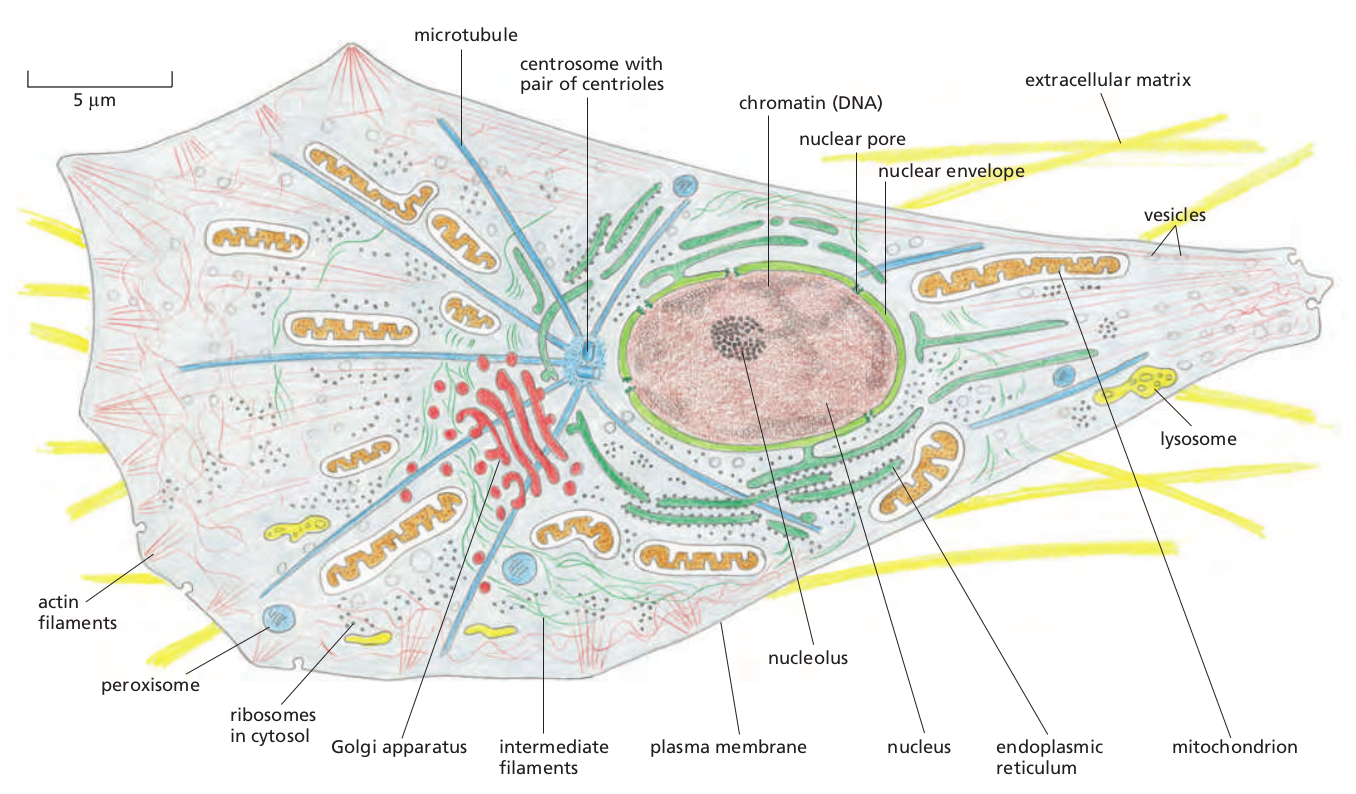
\includegraphics[width=0.5\textwidth]{celula_eucariota}}
  \subfloat[Dogma central de la biología molecular]{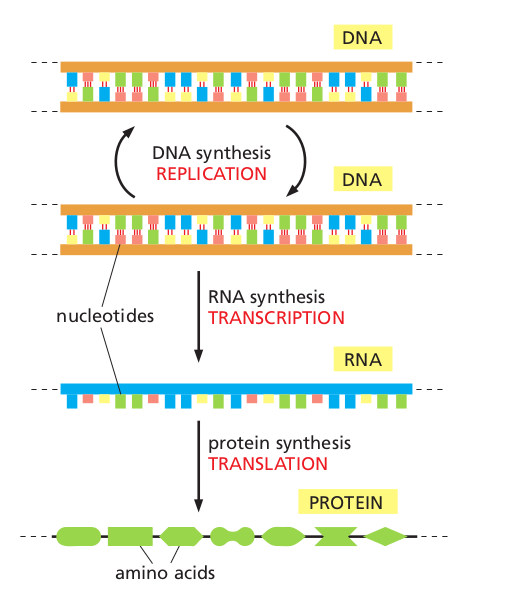
\includegraphics[width=0.5\textwidth]{adn3}}
\end{figure}

\end{frame}

\subsubsection*{Cambios transcripcionales}
\begin{frame}
	\frametitle{Cambios transcripcionales en respuesta a estrés abiótico en \textit{A. thaliana}} 
	\begin{columns}[T]
		\column{0.5\textwidth}
			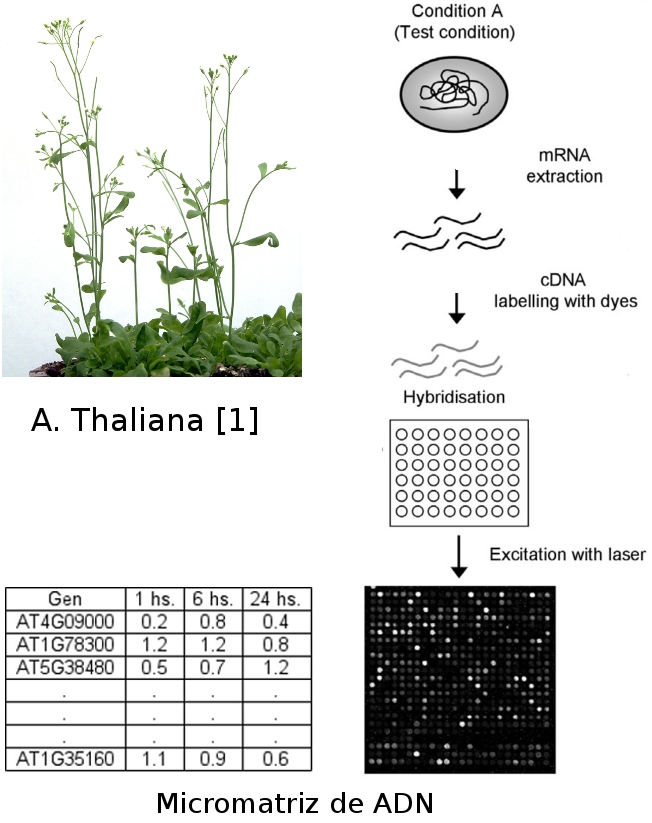
\includegraphics[width=1\textwidth]{micromatriz_y_arabidopsis}
		\column{0.5\textwidth}
			\bigskip
			\Large 
			Datos de estrés abiótico:
			\medskip
			\begin{itemize}
				\item 11 tratamientos
				\item $\approx 22000$ genes
				\item entre 4 y 8 mediciones temporales por gen y por tratamiento 
			\end{itemize}			
			\centering	
			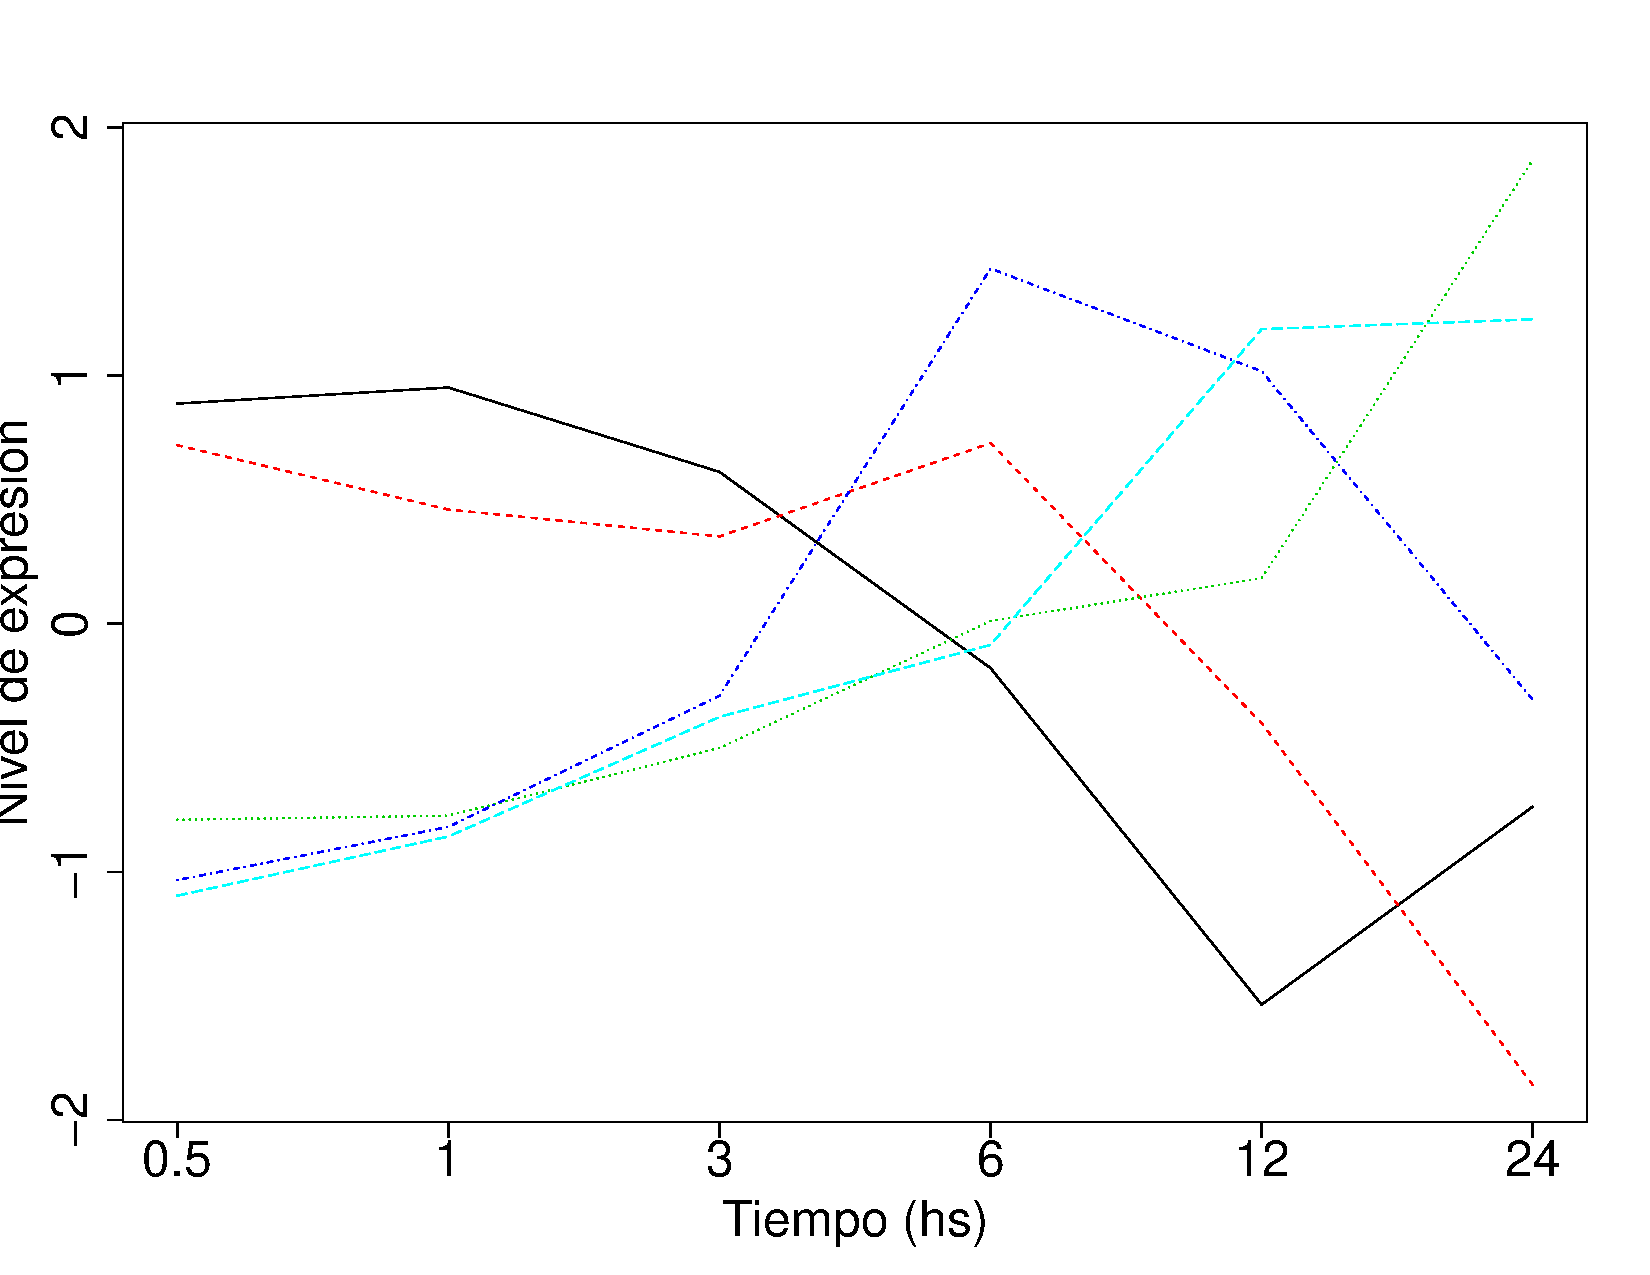
\includegraphics[width=0.9\textwidth]{perfiles_sin_agrupar.pdf}			
	\end{columns}
\end{frame}

\section{Análisis de relevamientos transcripcionales}


\subsection{Medidas de similaridad y distancia}
\begin{frame} \frametitle{Medidas de similaridad y distancia} 
\centering
Necesitamos definir que significa que dos datos sean ``similares''\bigskip
\begin{columns}[T]
\column{0.45\textwidth}
	Distancia euclidiana en espacio de alta dimensionalidad:\\
	\begin{equation}
		d_{euc}(\vec{x}, \vec{y}) = [\sum\limits_{i=1}^n (x_i-y_i)^2]^\frac{1}{2}
	\end{equation}
	\bigskip
	\centering
	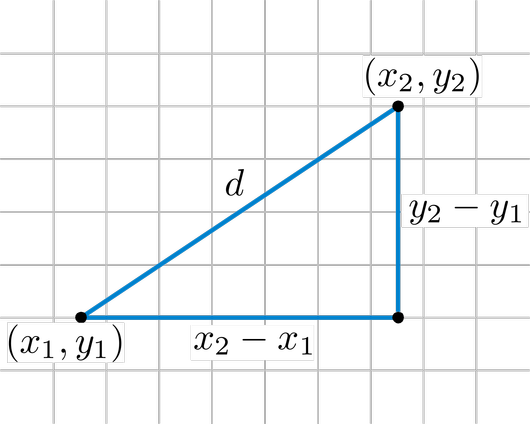
\includegraphics[width=0.7\textwidth]{distancia_euclidiana}

\column{0.55\textwidth}
	Distancia basada en el coeficiente de correlación de Pearson:\\
	\begin{equation}
		r(\vec{x}, \vec{y}) = \frac{\frac{1}{n-1}\sum\limits_{i=1}^n(x_i-\bar{x})(y_i-\bar{y})}{s_x s_y}
	\end{equation}
	\begin{equation}
		d_{ccp}(\vec{x}, \vec{y}) = 1-r(\vec{x}, \vec{y})
	\end{equation}
	\centering	
	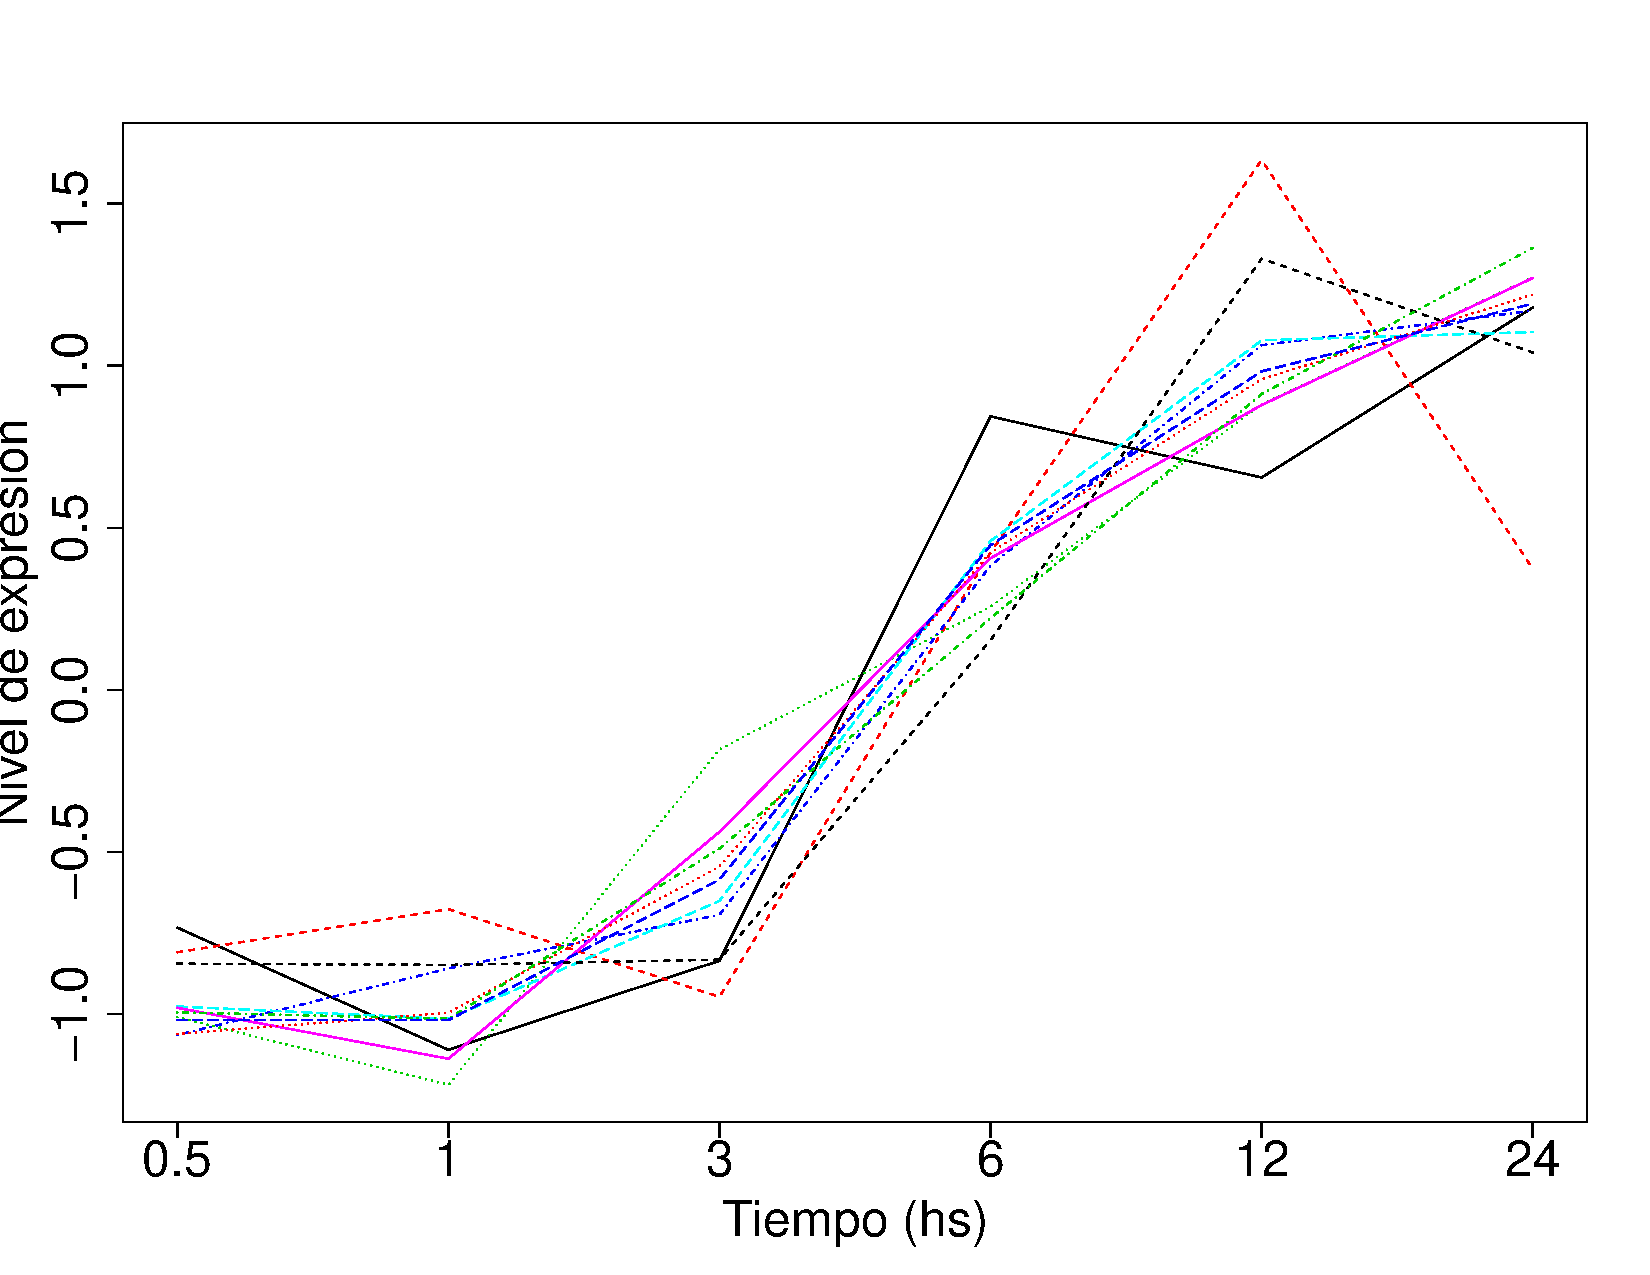
\includegraphics[width=0.7\textwidth]{perfiles_coregulados.pdf}
\end{columns}

\end{frame}

\subsection{Tipos de agrupamiento}
\begin{frame}
\frametitle{Tipos de agrupamiento} 
\end{frame}

\subsection{Métodos utilizados}
\begin{frame}
\frametitle{Métodos k-means, corte de árbol dinámico} 
\end{frame}

\subsection{Caracterización de particiones}
\begin{frame}
\frametitle{Caracterización de particiones} 
\end{frame}

\subsection{El problema de la escala}
\begin{frame}
\frametitle{El problema de la escala} 
\end{frame}

\section{Congruencia biológica}

\subsection{Ontología génica (GO)}
\begin{frame}
\frametitle{Ontología génica (GO)} 
\end{frame}

\subsection{Densidades de interacción}
\begin{frame}
\frametitle{Densidades de interacción} 
\end{frame}

\subsection{Indice de homogeneidad biológica}
\begin{frame}
\frametitle{Indice de homogeneidad biológica} 
\end{frame}

\section{Coherencia entre métricas}
\begin{frame}
\frametitle{Coherencia entre métrica transcripcional y espacio GO} 
\end{frame}

\subsection{KTA global}
\begin{frame}
\frametitle{KTA global} 
\end{frame}

\subsection{Modulación de heterogeneidades
transcripcionales}
\begin{frame}
\frametitle{KTA local para modulación de heterogeneidades transcripcionales} 
\end{frame}
\subsubsection*{Métrica mixta}
\begin{frame}
\frametitle{Métrica mixta} 
\end{frame}
\subsubsection*{Método heurístico}
\begin{frame}
\frametitle{Método heurístico} 
\end{frame}
\subsubsection*{Interpretación biológica}
\begin{frame}
\frametitle{Interpretación biológica} 
\end{frame}
\section{Conclusiones y perspectivas}
\begin{frame}
\frametitle{Conclusiones y perspectivas} 
\end{frame}
\end{document}